\chapter{Planificación temporal y estimación de costes}
\label{chap:planificacion}

Tan importante como la estimación económica del proyecto es la planificación temporal del mismo. La duración de cada activida del proyecto vendrá dada por múltiples factores entre ellos la complejidad, el esfuerzo requerido y el tiempo disponible.

Del equilibrio entre ambos factores depende en buena parte la viabilidad del
proyecto. Por ello, es necesario realizar un estudio del tiempo que se va a dedicar a cada fase y un análisis económico. Una buena gestión maximiza la probabilidad de consecución de resultados a tiempo, dentro de presupuesto y con la calidad esperada.

A continuación se presenta la planificación temporal y la estimación de costes de nuestro proyecto.

\section{Fases del proyecto} 

La planificación se ha realizado desglosando el proyecto en seis fases o tareas: análisis, diseño, codificación, pruebas, documentación y memoria. 

La duración de cada actividad del proyecto viene dada por múltiples factores, entre ellos la curva de aprendizaje de las tecnologías utilizadas para cada actividad, la complejidad de los problemas a resolver y los contratiempos que han surgido en cada etapa.

Para la realización del proyecto, por circunstancias personales se ha establecido un horario de 28 horas semanales, salvo para el último mes que han sido de 40 horas semanales. En aquellos casos en que las actividades se solapan, para facilitar los cálculos, se ha supuesto que el tiempo dedicado a cada una de ellas ha sido equivalente. Cada cuadro sombreado de la gráfica corresponde aproximadamente a una semana de trabajo (figura \ref{fig:planificacion}, página \pageref{fig:planificacion})


\begin{figure}[H]
  \centering
  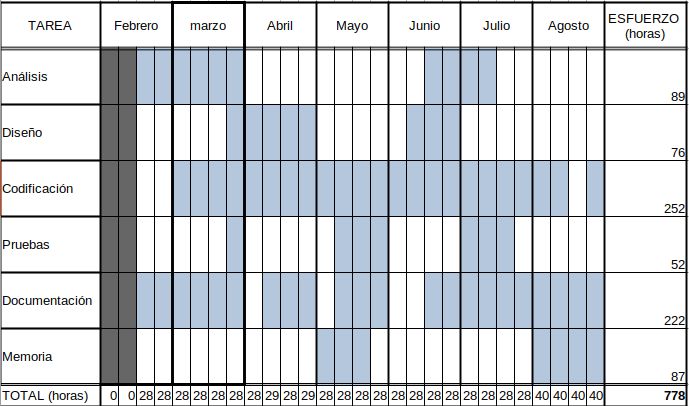
\includegraphics[width=0.50\textwidth]{imaxes/planificacion.png}
  \caption{Tabla de tiempos de planificación del proyecto}
  \label{fig:planificacion}
\end{figure}


\section {Costes estimados}

Este trabajo ha requerido aproximadamente 777 horas de trabajo personal que
podríamos valorar en 13.986 € a razón de 18 €/hora. A este coste habría que añadir el coste del esfuerzo dedicado por el director del proyecto, software, equipo, y otros gastos generales como electricidad, conexión a Internet, etc.

Si el proyecto fuese llevado a cabo por un equipo multidisciplinar, el coste laboral total dependería de la categoría de cada integrante atendiendo a su cualificación profesional. Podría estar formado por:
\begin{itemize}
\item Consultor, que se encarga de las líneas de investigación del
departamento.
\item Ingeniero Senior, con funciones de dirección de proyecto.
\item Ingeniero Junior, con una experiencia menor de cinco años.
\item Técnicos Informáticos.
\item Personal Auxiliar.
\end{itemize}

A los costes laborales habría que añadir los derivados de:
\begin{itemize}
\item Material y equipo (hardware, licencias, consumibles, conexión a
Internet, etc.).
\item Costes generales (luz, teléfono, impuestos).
\item Otros gastos no reflejados en los apartados anteriores.
\end{itemize}
